\section{Experimental Procedure}

The goal is to determine the maximum resolution of a microscope.

The experiment will be split into three experiments:

\begin{enumerate}
	\item{Experiment: Calculating the magnification by measuring the tube optimal length}
	\item{Experiment: Determining the lattice constant d by measuring the width of the gap and the thickness of a grid-wire}
	\item{Experiment: Determining the maximum resolution of the microscope by using an adjustable pinhole.}
\end{enumerate}

For the first experiment a microscope was prepared as shown in illustration 1.  The goal was to find the right tube length to match the calculated magnification. A lamp with a scale was placed at the end, which emitteds alight at a wavelength of 550nm. The objective lens ($f_{ok}$ = 50mm) was placed some distance behind the lamp. Behind the objective lens the ocular lens ($f_{ob}$=50mm) was placed. The tube had a length of 100mm. A semi-transparent mirror was placed in front of the ocular at a 45° angle, which reflected a second scale (same size as the scale on the lamp). The distance between the object and the second scale had to be $s_{0}$=250mm. It was also necessary to keep the distance from the ocular to the eye at $s_{0}$, to see a clear image.
\\
By trial and error, the optimal distance x=25cm from the lamp to the objective lens was found. At this point the theoretical magnification (equation X) and the measurement (equation X) cwere bothe equal to two. The magnification was calculated using equation X. To check the correctness, the experiment was repeated twice more (x=25cm ) with the tube length changed to 150mm and 200mm.

\begin{figure}[h!]
    \centering
  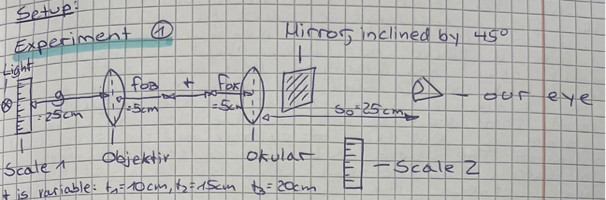
\includegraphics[]{Illu1_Experiment_setup_1.jpg}
  \caption{Setup of experiment 1(Leander Koufen)}
\end{figure}

In experiment 2 a grid was now placed in front of the lamp and the tube length changed to 300mm to get a sufficient magnification. An ocular micrometre (graduation: 1,33 $\pm$ 0,06 $\cdot10^{-9}$ mm) in the focal point of the ocular lens was needed to measure the gaps and the thickness of the wires from the grid.

As last step of the experiment, the ocular micrometre was switched with an adjustable pinhole. By changing the pinhole size, it was possible to determine the resolution limit.

\begin{figure}[h!]
    \centering
  \includegraphics[]{Illu2_Experiment_setup_3.jpg}
  \caption{Setup of experiment 3(Leander Koufen)}
\end{figure}

\newpage
